\section{PhaistOS, le générateur d'ordonnanceurs d'E/S}
\label{intro}

\subsection{Quésaco}

``PhaistOS'' est le nom d'un Langage Dédié, ou Domain Specific Language (DSL) en anglais. Utilisé dans le domaine de l'ordonnancement des entrées/sorties (E/S) d'un système d'exploitation (SE), il a pour but de faciliter la conception et la validation des politiques d'E/S écrite par un utilisateur. Il est le fruit issu du projet VeriAMOS (Verified Abstract Machines for Operating Systems) ayant pour but de s'attaquer au problème de vérification d'une classe de services de systèmes d'exploitation.

\subsection{La structure d'accueil}

Mon stage a donc porté sur le projet VeriAMOS, au sein de l'équipe Erods, accompagnée par les équipes Antique (INRIA Paris) et Whisper (Université de Sorbonne). Erods est une équipe de laboratoire qui étudie principalement la construction et la gestion de sytèmes cloud, en travaillant sur différentes facettes de ces derniers, comprenant la prise en charge d'environement d'execution distribué robuste et efficace. 

Erods fait donc parti du Laboratoire d'Informatique de Grenoble (LIG) avec 23 autres équipes réparties sur 5 axes de recherches (voir Figure~\ref{fig:lig}). Ce laboratoire, reconnu internationalement, se base sur les sciences informatiques et cherche à approfondir ses concepts, allant jusqu'à la réalisation de maquettes innovantes qui anticipent les usages. Le laboratoire de recherche universitaire se situe sur le campus grenoblois de Saint Martin d'Hères (Université Grenoble Alpes (UGA)) et est composé de 500 chercheurs et enseignants chercheurs.

\begin{figure}[h!t] \centering
    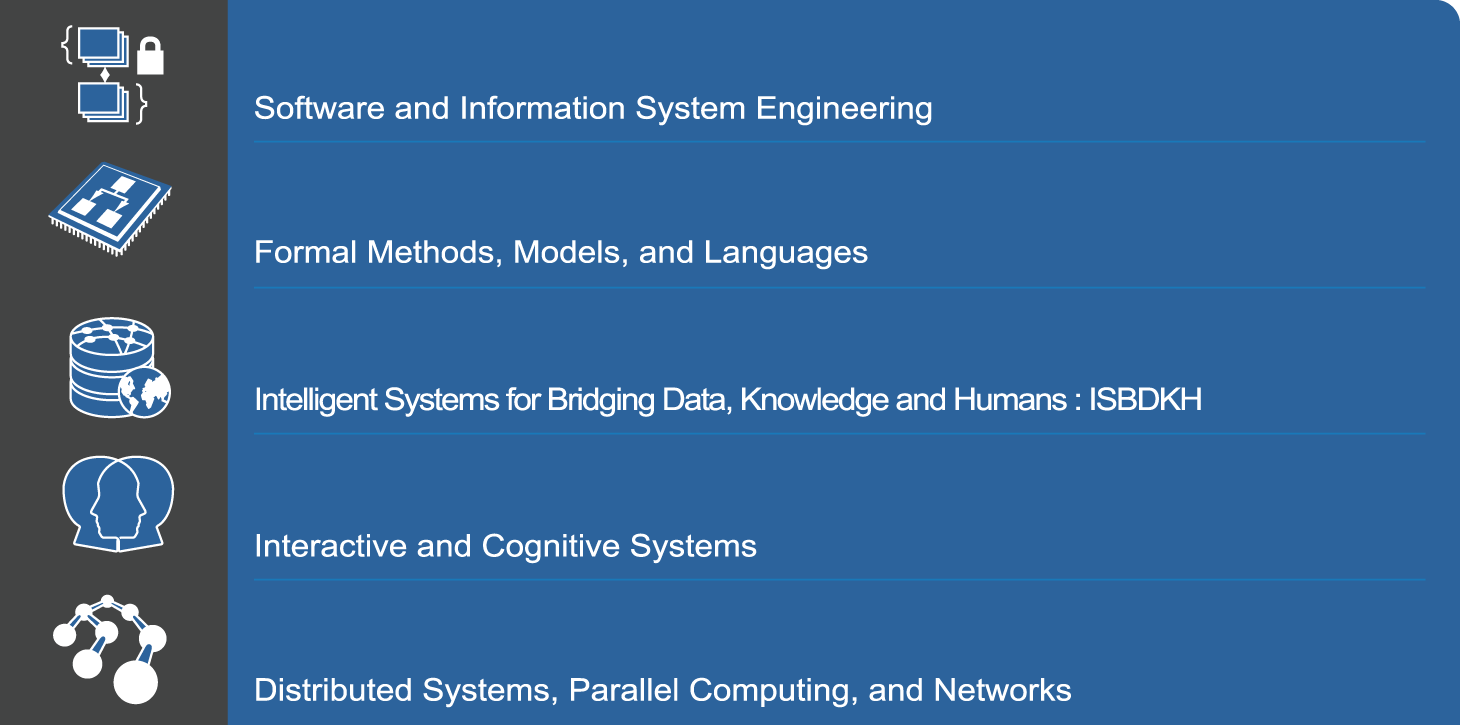
\includegraphics[width=12.5cm]{images/axeslig}
    \caption{Les différents axes de recherche du LIG.}
    \label{fig:lig}
\end{figure}

Mon employeur officiel reste donc l'université, c'est-à-dire l'UGA. Mon équipe et moi-même étions localisé sur le campus, plus précisément dans le bâtiment ``IMAG'', au quatrième étage consacré à la recherche dans le domaine informatique (voir mon bureau sur la Figure~\ref{fig:imag}).

\begin{figure}[h!t] \centering
    \begin{tabular}{@{}c@{\hspace{5pt}}c@{}}
    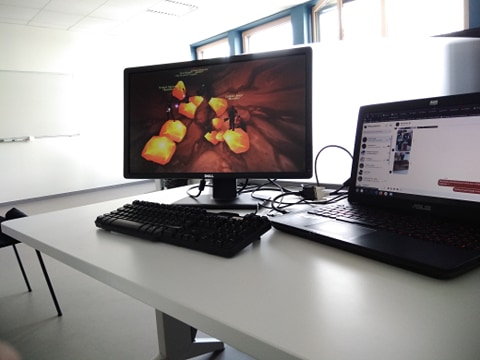
\includegraphics[width=0.49\textwidth]{images/desk} & 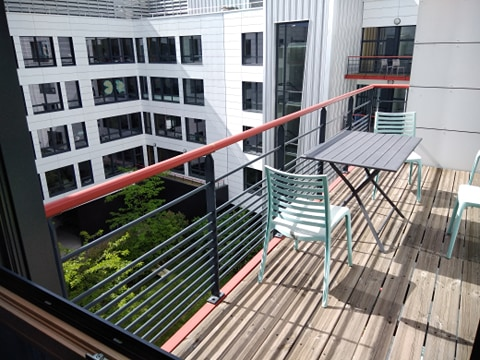
\includegraphics[width=0.49\textwidth]{images/balcony}
    \end{tabular}
    \caption{Bureau de travail et balcon vu de la fenêtre.}
    \label{fig:imag}
\end{figure}

\subsection{Pourquoi PhaistOS ?}

Pour revenir sur le sujet de stage et le comprendre il faut tout d'abord expliquer pourquoi VeriAMOS à lieu d'être. En effet ce projet à pour but d'améliorer la vérification de systèmes d'exploitation, qui reste aujourd'hui compliqué pour deux raisons principales. Premièrement, les propriétés mathématiques des algorithmes sous-jacents sont généralement difficiles à exprimer, deuxièmement, la structure du code qui implémente ces algorithmes dans le SE est en général très complexe. 

Afin d'éviter de se retrouver dans cette situation d'un niveau de difficulté trop élevé, VeriAMOS propose d'utiliser une technique d'abstraction basée sur un DSL (comme le fait Bossa~\cite{Barreto-Muller:asf2002}), ainsi qu'un analyseur statique, qui, à froid, pourra vérifier un ensemble de services fournis par le SE, comme par exemple celui de l'ordonnanceur des requêtes d'E/S.

Dans cette approche de développement système, le programme écrit avec le langage du DSL pourra être compilé pour générer un code source dans le langage du système et qui implémente le service visé (plus de détails Partie~\ref{context}). En limitant ainsi la capacité d'expression du langage, le DSL contraint le programmeur et permet d'éviter une mauvaise utilisation des outils du langage cible, permettant ainsi d'améliorer la robustesse des services concernés du SE. Le développeur pourra donc se focaliser sur l'écriture de sa politique système de haut niveau et déléguera la génération de code au compilateur du DSL.

VeriAMOS offre une opportunité de formaliser et d'implémenter une nouvelle approche à la vérification de systèmes d'exploitation, sur différents services. Ici nous nous focaliserons sur celui de l'ordonnanceur d'E/S du système, mais nous pensons que cette approche reste générale et pourrait s'appliquer sur tout types d'ordonnanceurs, de systèmes de fichier, etc.

\subsection{Mon rôle dans ce projet}

Concernant le projet, la mission qui m'a été attribuée porte uniquement sur la partie compilateur de PhaistOS, j'ai donc du me familiariser avec le DSL et son implémentation.